\documentclass[paper=a4, fontsize=13pt]{extarticle} % A4 paper and 11pt font size
\usepackage{longtable} % Allows tables to span multiple pages (this package must be called before hyperref)
\usepackage{natbib}
\bibliographystyle{chicago}
\renewcommand{\familydefault}{\rmdefault}
\usepackage{lmodern}
\usepackage[T1]{fontenc} % Use 8-bit encoding that has 256 glyphs
\usepackage{fourier} % Use the Adobe Utopia font for the document - comment this line to return to the LaTeX default
\usepackage[english]{babel} % English language/hyphenation
\usepackage{amsmath,amsfonts,amsthm,tikz} % Math packages
\usepackage{multicol}
\usepackage{graphicx}
\usepackage{lipsum} % Used for inserting dummy 'Lorem ipsum' text into the template
\usepackage{subfigure}
\usepackage{here}
\usepackage{setspace}
\usepackage{amssymb}
\usepackage{wasysym}
\usepackage[center]{caption}
\usepackage[hidelinks]{hyperref}

\usepackage{multirow}

\usepackage{array}
\newcolumntype{L}[1]{>{\raggedright\let\newline\\\arraybackslash\hspace{0pt}}m{#1}}
\newcolumntype{C}[1]{>{\centering\let\newline\\\arraybackslash\hspace{0pt}}m{#1}}
\newcolumntype{R}[1]{>{\raggedleft\let\newline\\\arraybackslash\hspace{0pt}}m{#1}}

\usepackage{xcolor}
\hypersetup{
    colorlinks,
    linkcolor={red!50!black},
    citecolor={blue!50!black},
    urlcolor={blue!80!black}
}
\newcommand\independent{\protect\mathpalette{\protect\independenT}{\perp}}
\def\independenT#1#2{\mathrel{\rlap{$#1#2$}\mkern2mu{#1#2}}}
\newtheorem{proposition}{Proposition}
\newtheorem{mydef}{Definition}
\newtheorem{lemma}{Lemma}
\newtheorem{thm}{Theorem}
\newtheorem{corollary}{Corollary}
\newtheorem{ass}{Assumption}
\newtheorem{nota}{Notation}
\usepackage{fullpage}
\onehalfspacing
\allowdisplaybreaks

\numberwithin{equation}{section} % Number equations within sections (i.e. 1.1, 1.2, 2.1, 2.2 instead of 1, 2, 3, 4)
\numberwithin{figure}{section} % Number figures within sections (i.e. 1.1, 1.2, 2.1, 2.2 instead of 1, 2, 3, 4)
\numberwithin{table}{section} % Number tables within sections (i.e. 1.1, 1.2, 2.1, 2.2 instead of 1, 2, 3, 4)

%\newcommand\independent{\protect\mathpalette{\protect\independenT}{\perp}}
\def\independenT#1#2{\mathrel{\rlap{$#1#2$}\mkern2mu{#1#2}}}
\newcommand{\btz}{\begin{tikzpicture}}
\newcommand{\etz}{\end{tikzpicture}}
\usetikzlibrary{snakes}

\usepackage{enumitem}
\setlist[enumerate]{itemsep=0mm}

\usepackage{pdflscape}

\usepackage{booktabs}
\usepackage{adjustbox}
\usepackage{libertine}% Linux Libertine, may favourite text font
\usepackage[euler-digits]{eulervm}% A pretty math font
\usepackage{dcolumn} % Align on the decimal point of numbers in tabular columns
     \newcolumntype{d}[1]{D{.}{.}{#1}}
\usepackage{xhfill}
\newcommand{\ditto}[1][.4pt]{\xrfill{#1}~\textquotedbl~\xrfill{#1}}
\usepackage{threeparttable} % For better formatting of table notes
%\usepackage{parskip}
\usepackage{longtable}
\usepackage{threeparttablex}
\usepackage{dcolumn}

\newcommand{\sym}[1]{\rlap{#1}}% Thanks to David Carlisle

\let\estinput=\input% define a new input command so that we can still flatten the document

\newcommand{\estwide}[3]{
		\vspace{.75ex}{
			\begin{tabular*}
			{\textwidth}{@{\hskip\tabcolsep\extracolsep\fill}l*{#2}{#3}}
			\toprule
			\estinput{#1}
			\bottomrule
			\addlinespace[.75ex]
			\end{tabular*}
			}
		}	

\newcommand{\estauto}[3]{
		\vspace{.75ex}{
			\begin{tabular}{l*{#2}{#3}}
			\toprule
			\estinput{#1}
			\bottomrule
			\addlinespace[.75ex]
			\end{tabular}
			}
		}

% Allow line breaks with \\ in specialcells
	\newcommand{\specialcell}[2][c]{%
	\begin{tabular}[#1]{@{}c@{}}#2\end{tabular}}

\newcommand{\figtext}[1]{
	\vspace{-1.9ex}
	\captionsetup{justification=justified,font=footnotesize}
	\caption*{\hspace{6pt}\hangindent=1.5em #1}
	}
\newcommand{\fignote}[1]{\figtext{\emph{Note:~}~#1}}

\newcommand{\figsource}[1]{\figtext{\emph{Source:~}~#1}}

% Add significance note with \starnote
\newcommand{\starnote}{\figtext{* p < 0.1, ** p < 0.05, *** p < 0.01. Standard errors in parentheses.}}

\usepackage{siunitx} % centering in tables
	\sisetup{
		detect-mode,
		tight-spacing	        	  = true,
		group-digits	        	  = false ,
		input-signs		              = ,
		input-symbols	 	        = ( ) [ ] - + *,
		input-open-uncertainty	= ,
		input-close-uncertainty	 = ,
		table-align-text-post	  = false
        }
\newcommand{\horrule}[1]{\rule{\linewidth}{#1}} % Create horizontal rule command with 1 argument of height
\definecolor{olivegreen}{cmyk}{0.28,0,0.5,0.68}
\usepackage{listings}
\lstset{language=R,
    basicstyle=\small\ttfamily,
    stringstyle=\color{olivegreen},
    %otherkeywords={0,1,2,3,4,5,6,7,8,9},
    morekeywords={TRUE,FALSE,fminbnd,optim,optimize,fzero},
    deletekeywords={data,frame,length,as,character},
    keywordstyle=\color{blue},
    commentstyle=\color{olivegreen},
}

\author{Yujung G. Hwang} % Your name
\date{\today} % Today's date or a custom date

\begin{document}

\title{	
\normalfont \normalsize 
\huge Problem Set 3 Solution
}
\author{
Instructor : Yujung Hwang \thanks{\texttt{yujungghwang@gmail.com}}} % Your name
\date{\today} % Today's date or a custom date
\maketitle % Print the title

\upshape \mdseries 

\normalsize

\textbf{Question 1} \\
(a) I use the mean asset from age 2 to T (exclude age 1 because there is no variation in asset at T=1), and regression coefficients from regressing consumption on income and asset from t=1 to t=T-1 (exclude t=T because people will consume everything on hand). I use the coefficient in front of income from age 1 to (T-1), and coefficient in front of asset from age 2 to (T-1) (exclude t=1 because there is no variation in asset at t=1). \\
Intuitively speaking, the average asset slope over life cycle captures both impatience and the rate of intertemporal substitution. The regression model approximates the structural consumption policy function. Both the functional form restriction and nonlinearity help parsing out $\beta$ and $\gamma$. \\

(b) It took 35 seconds.  \\

   user  system elapsed \\
 34.857   0.056  34.919 

(c) \\
\begin{lstlisting}
# try optimParallel for faster run
> oout <- optim(par=c(0.96,1.9),fn=getCriterionFunction,WeightMatrix=weightMat,lower=lb,upper=ub,
control=list(maxit=100),  method="L-BFGS-B")
> # print out estimate
> print(oout)
$par
[1] 0.9599982 1.8999468
\end{lstlisting}

(d) \\
\begin{lstlisting}
> dMoment <- jacobian(findMomentVec,oout$par) 
> covar <- (1+1/1)*solve(t(dMoment)%*%weightMat%*%dMoment)%*%t(dMoment)%*%weightMat%*%varMat%*%
weightMat%*%dMoment%*%solve(t(dMoment)%*%weightMat%*%dMoment)
> standerr <- sqrt(diag(covar))
> print(standerr)
[1] 0.00140486 0.03696738
\end{lstlisting}

(e) \\
The sensitivity measures show regression coefficients for income are critical for identifying beta and gamma. Beta is most sensitive to regression coefficient for income at t=1 and Gamma is most responsive to regression coefficient for income at t=T-1. The sensitivity to mean asset is close to 0, so does not help much identification. \\

\begin{figure}[H]
\centering
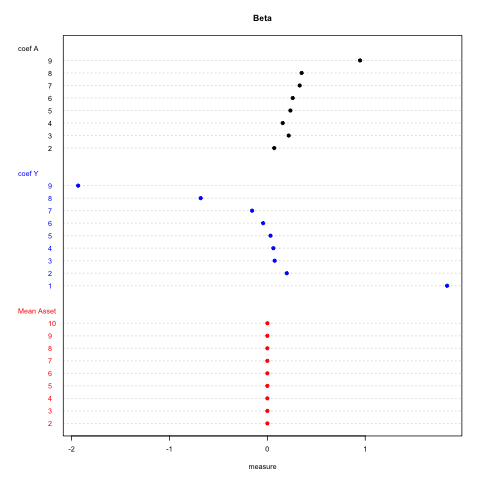
\includegraphics[width=0.6\linewidth]{BetaSensitivity}
\label{fig:betasensitivity}
\end{figure}
\begin{figure}[H]
\centering
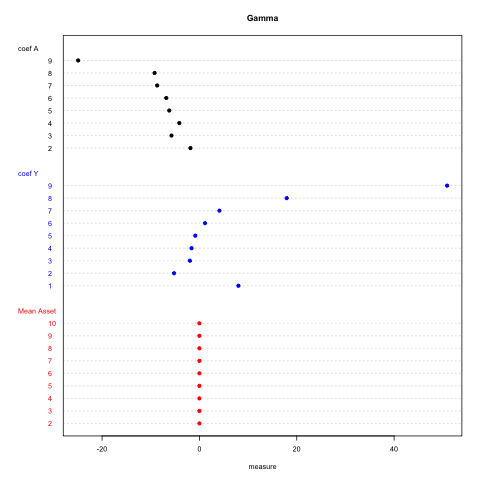
\includegraphics[width=0.6\linewidth]{GammaSensitivity}
\label{fig:gammasensitivity}
\end{figure}

(f) \\
The estimated parameter generates data which match actual data  very well. 

\begin{figure}[H]
\centering
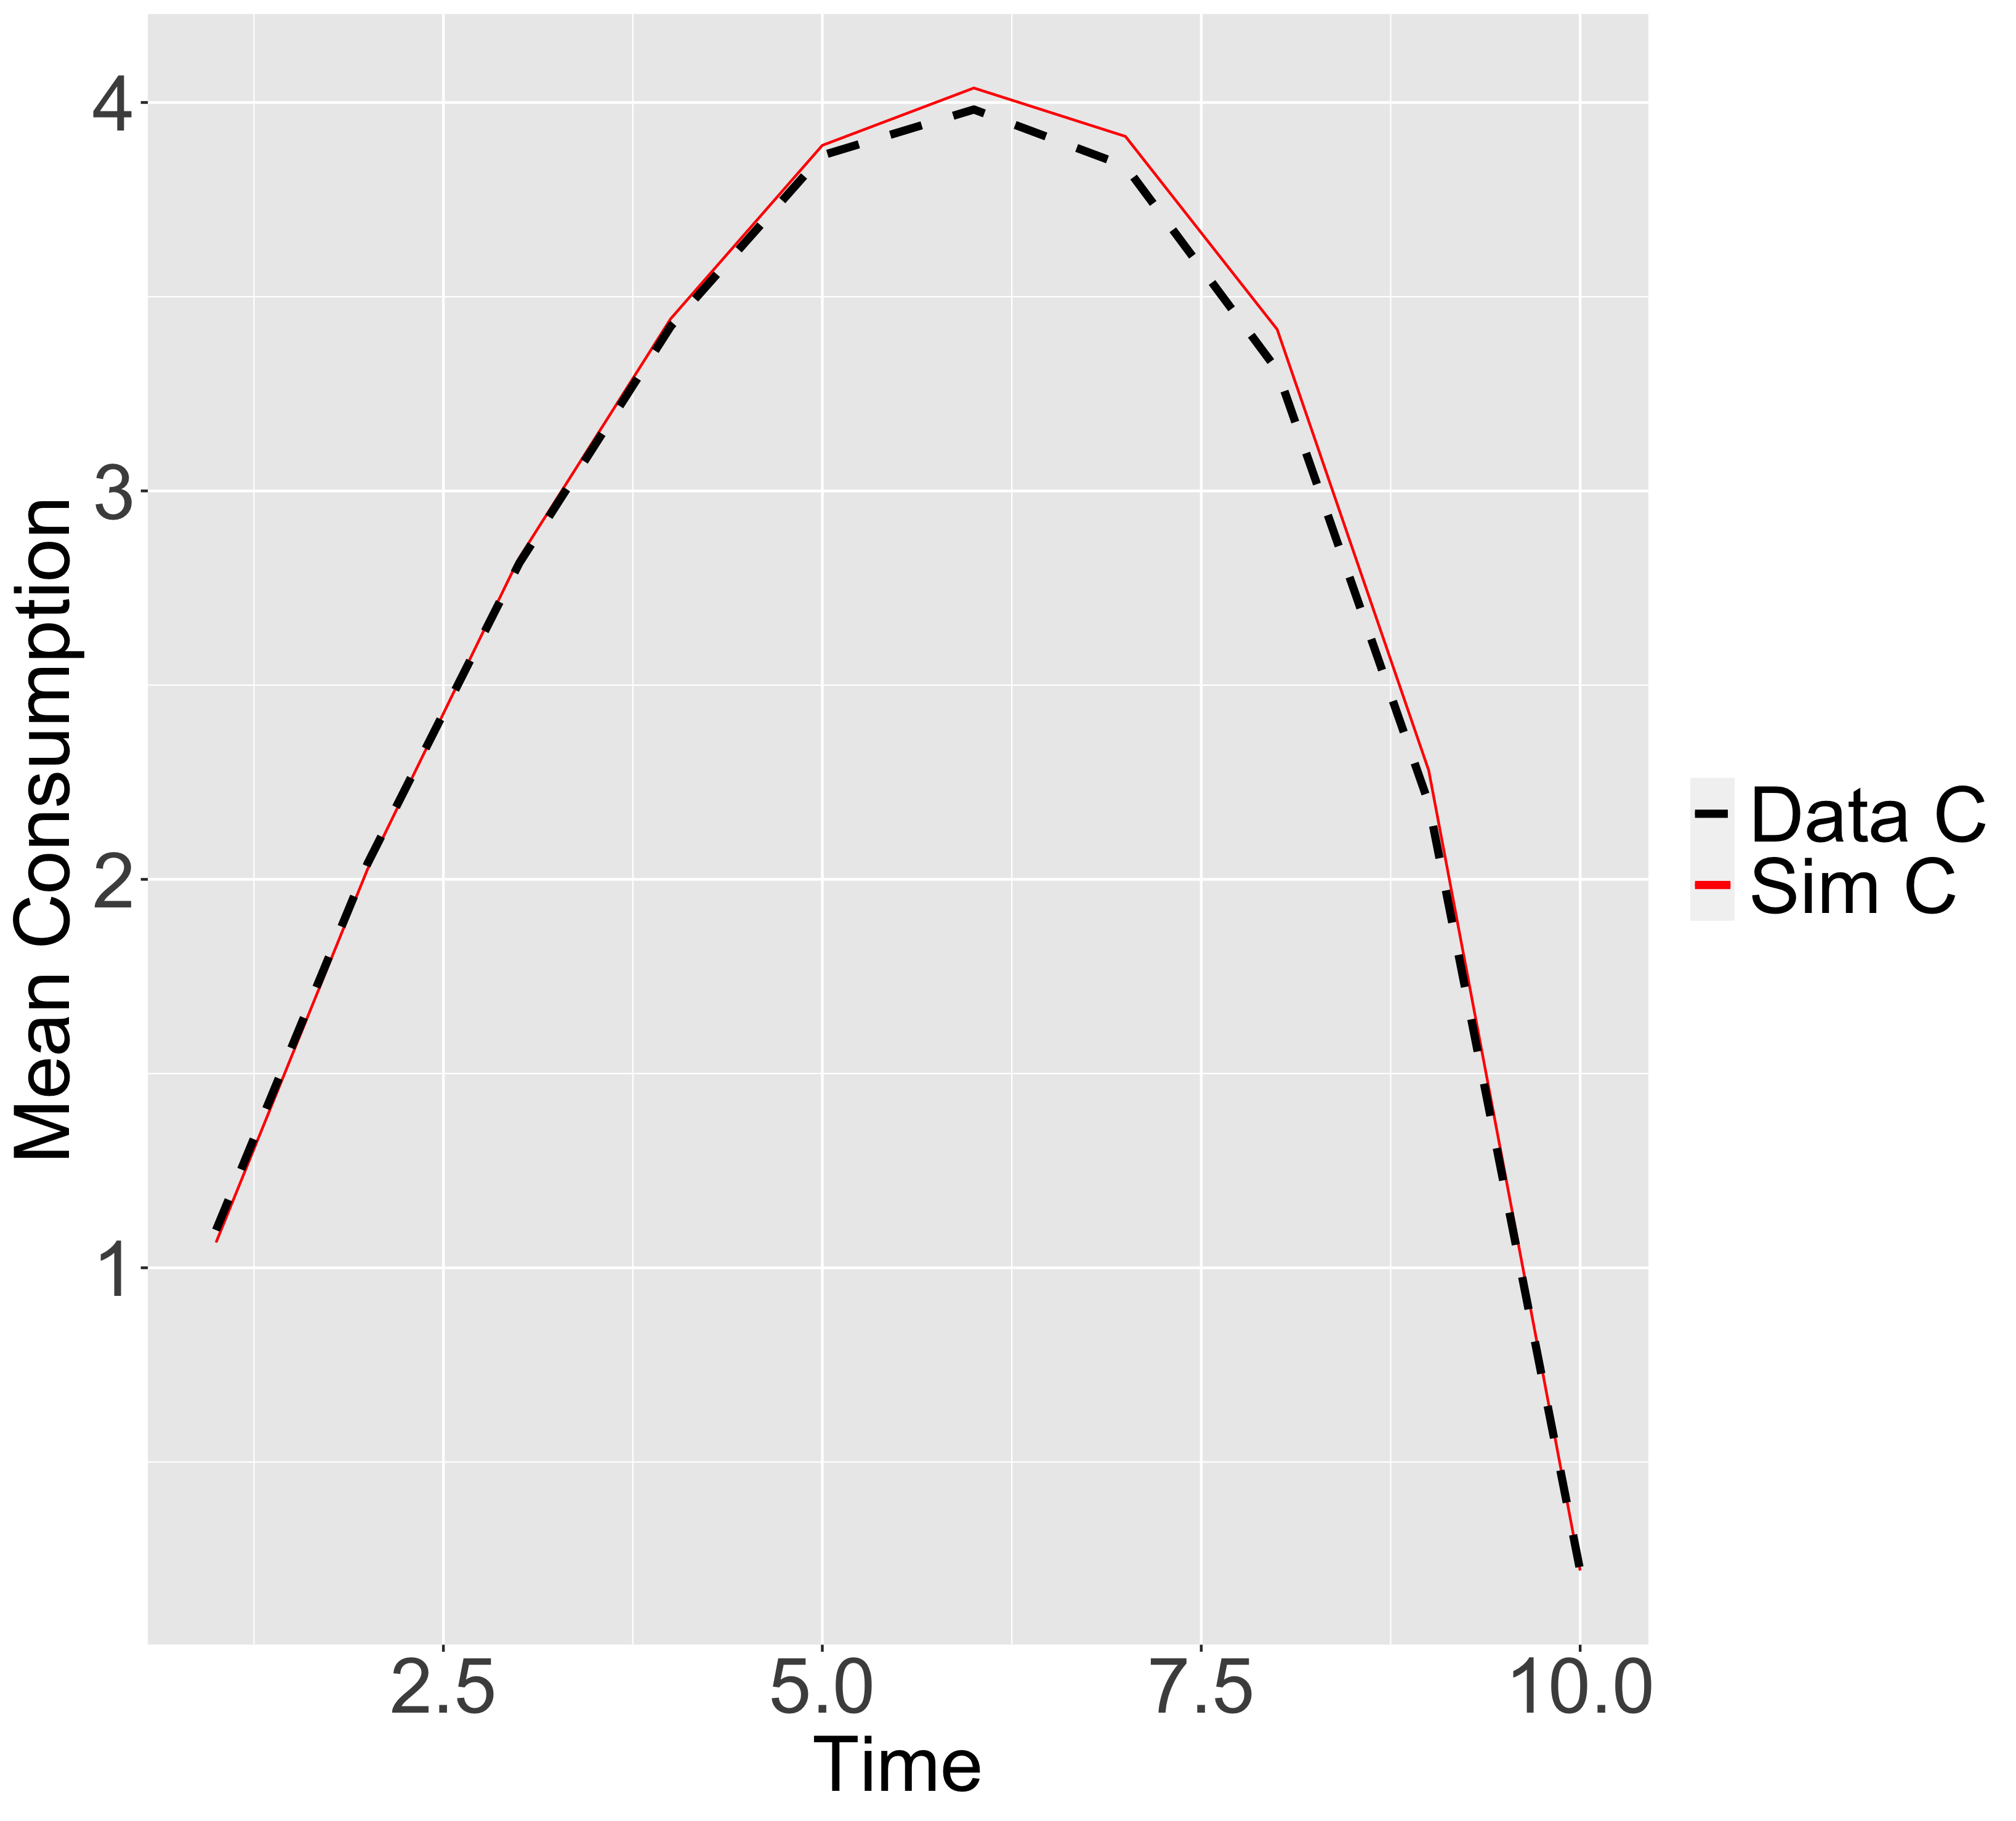
\includegraphics[width=0.6\linewidth]{modelFitCons}
\label{fig:modelfitcons}
\end{figure}
\begin{figure}[H]
\centering
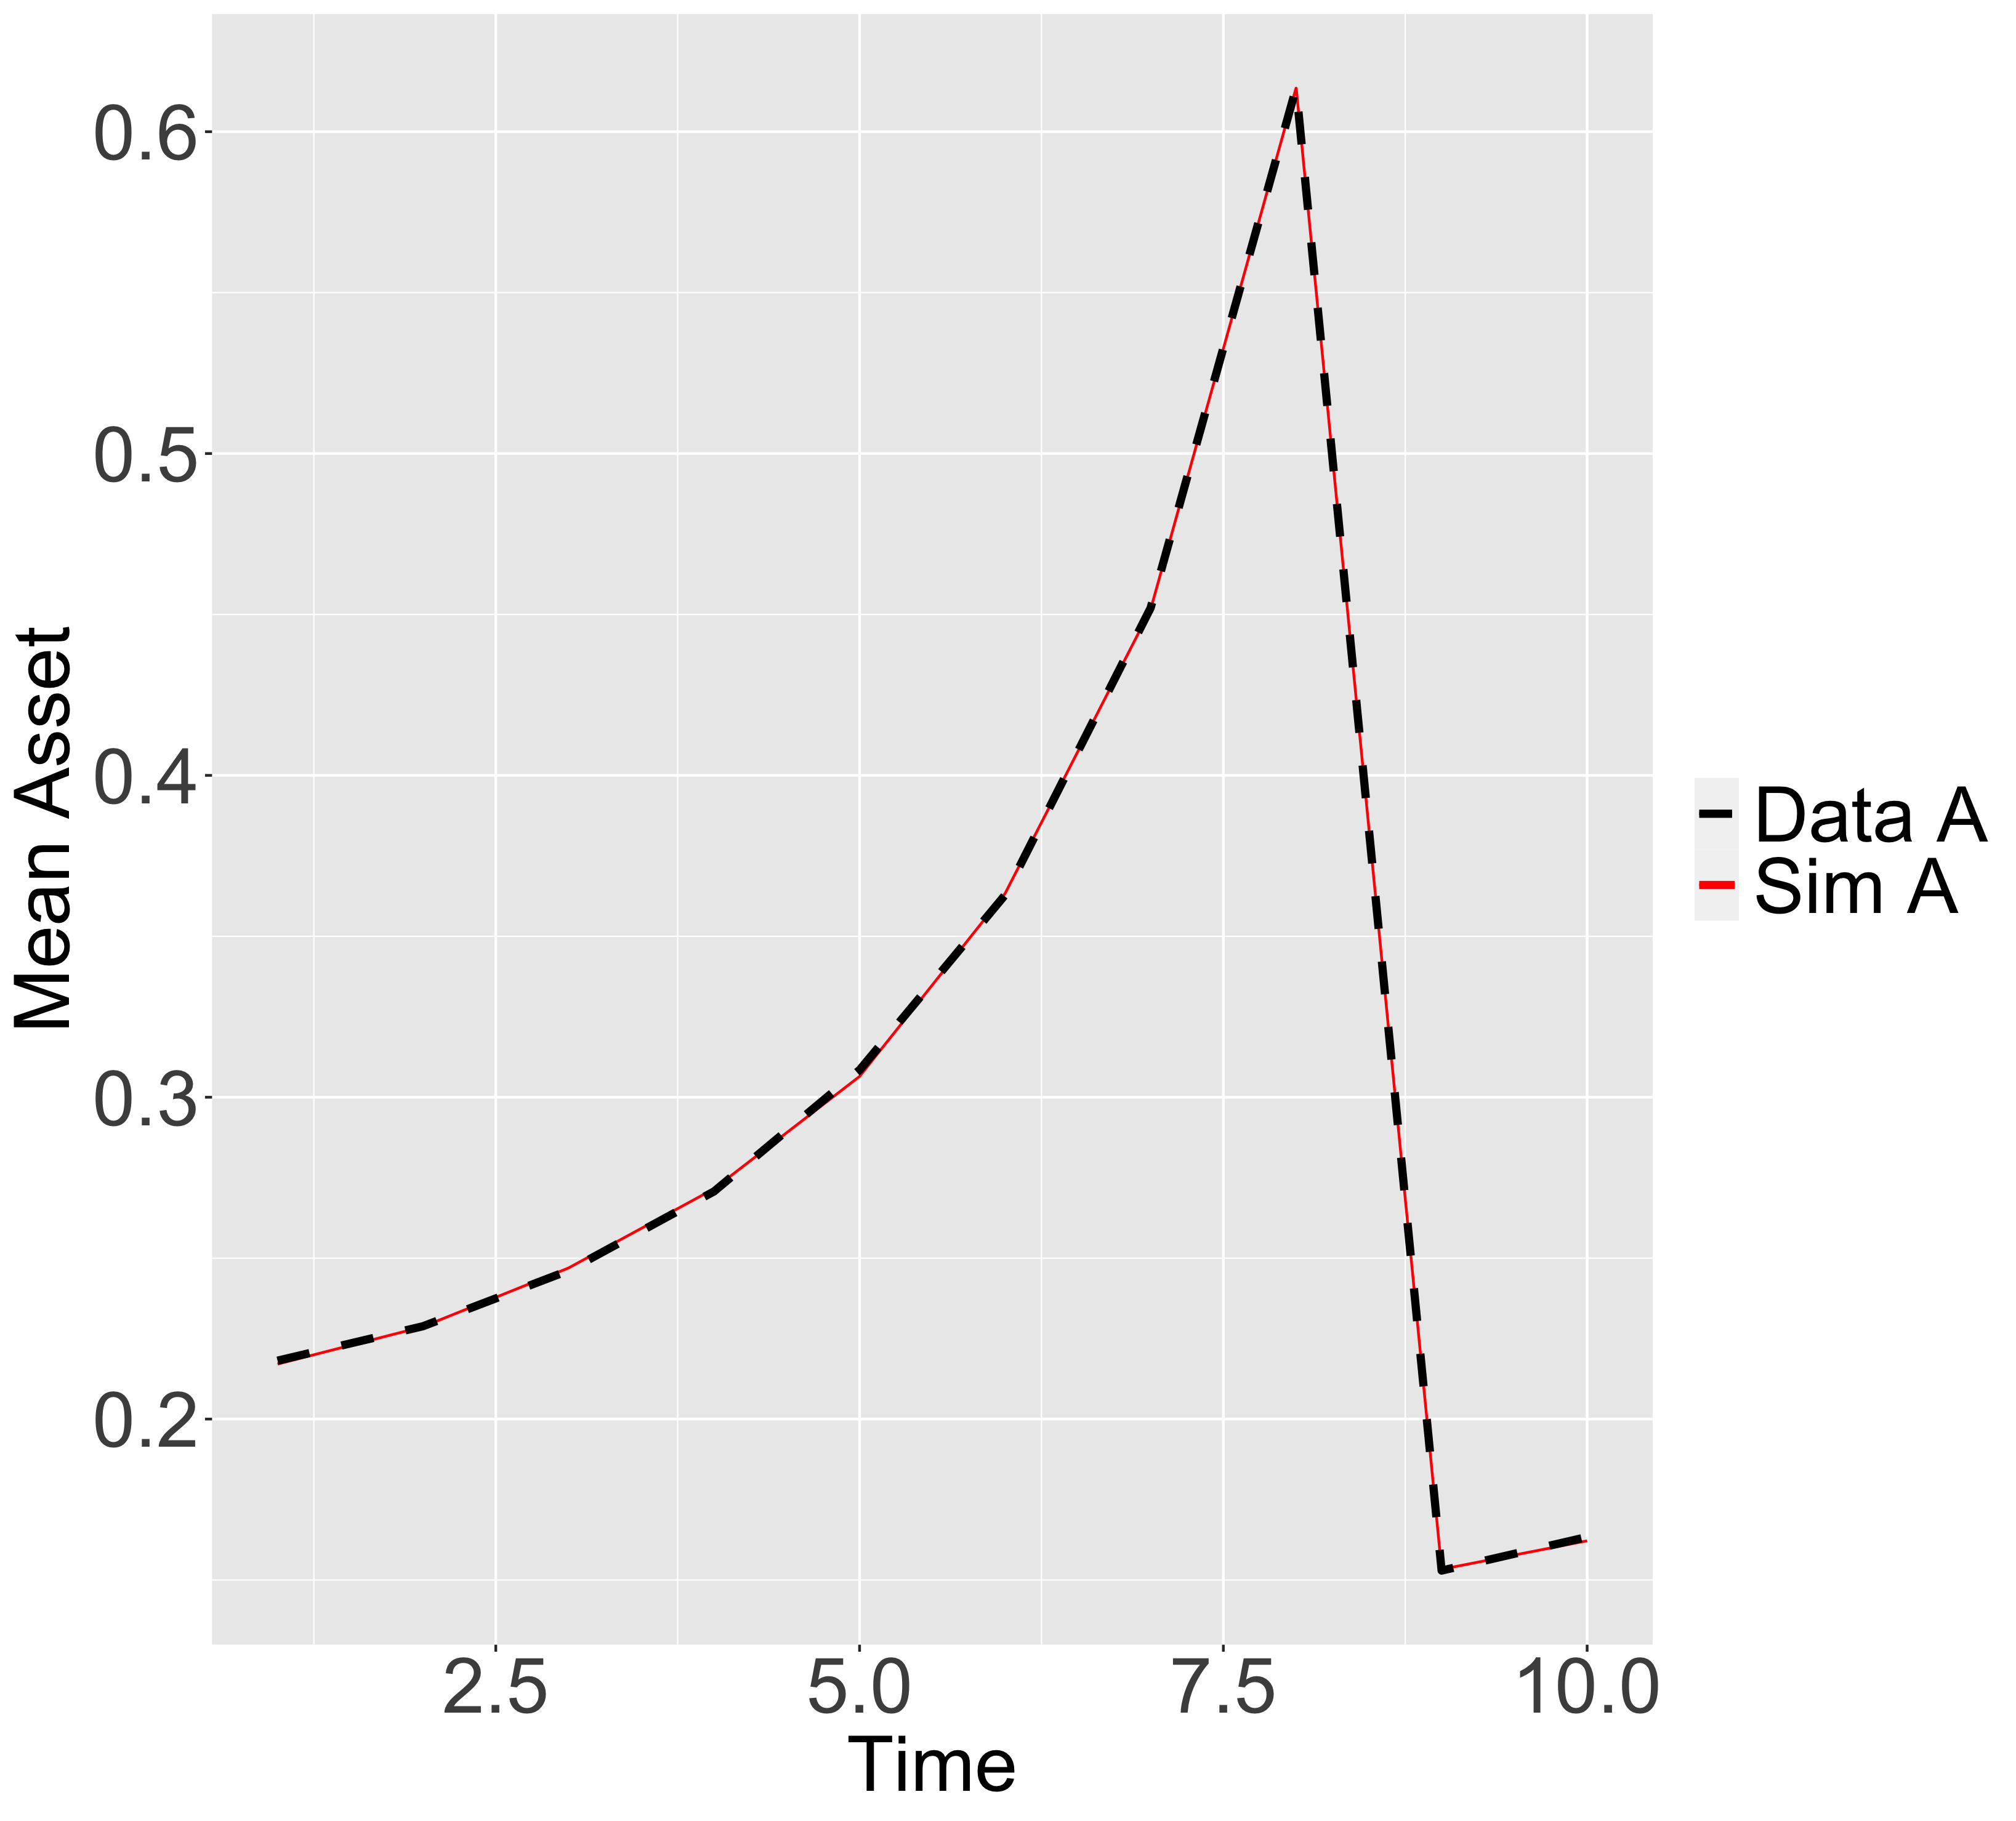
\includegraphics[width=0.6\linewidth]{modelFitAssets}
\label{fig:modelfitassets}
\end{figure}



\end{document}